\subsection{Additional antenna structures}\label{sec:add_antenna}

The monopole and loop antennas discussed in the previous sections represent the two fundamental reference cases for electric and magnetic dipole radiation, respectively. Their coupling behavior is governed by their dominant reactive character: the monopole antenna is capacitive, while the loop antenna is primarily inductive. This distinction proves to be the primary factor determining the equivalent dipole moments and their frequency dependence, rather than the specific antenna geometry.

The antennas investigated in the following sections can be understood as geometrical modifications of these reference cases, inheriting their respective reactive character. The loop antenna with a gap in the return path, discussed in \cref{sec:loop_gap_setup}, interrupts the current return path and thereby shifts the antenna toward capacitive behavior, yielding equivalent dipole moments analogous to those of the monopole antenna. The inverted-F and center-fed monopole antennas, investigated in \cref{sec:ifa_sim}, maintain a closed current path and exhibit predominantly inductive behavior, mirroring the results obtained for the loop antenna. The analysis in each case focuses on the deviations in the equivalent dipole moments and their frequency dependence relative to the respective reference structure, and identifies the geometrical modifications responsible for these differences.

\subsubsection{Loop antenna with gap}\label{sec:loop_gap_setup}
\FloatBarrier

\begin{figure}[htbp]
	\centering
	\begin{subfigure}[t]{0.48\textwidth}
		\centering
		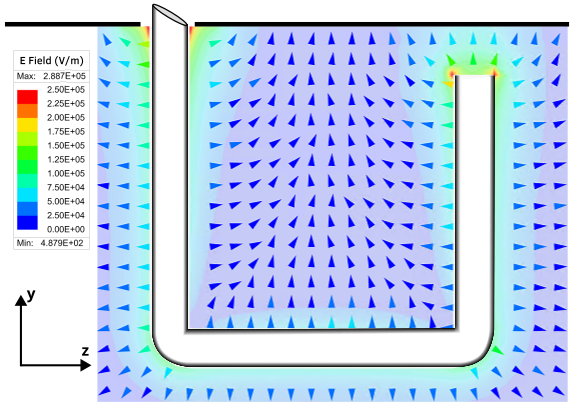
\includegraphics[width=1\linewidth]{content/img/gap_loop_antenna_fields}
		\caption{Electric near-field intensity}
		\label{fig:gaploopantennafields}
	\end{subfigure}
	\hfill
	\begin{subfigure}[t]{0.48\textwidth}
		\centering
		
\includegraphics[width=1\linewidth]{content/img/gapped_loop_antenna}
		\caption{Geometry of loop antenna with gap}
		\label{fig:gappedloopantenna}
	\end{subfigure}
	
	\caption{Geometry of the loop antenna in (a) with a gap in the return path inserted in the TEM cell, and its near-fields demonstrated in (b). The figure is not to scale.}
	\label{fig:gaploop}
\end{figure}

A loop antenna with a gap of height $10\,$µm introduced in the return path, as shown in \autoref{fig:gappedloopantenna}, is investigated to analyze the behavior of the generated dipole moments when the return path is interrupted. The gap is intentionally kept small to emphasize the relevant coupling mechanisms and to demonstrate the consistency of the antenna analysis within the framework developed in this thesis, even though such a dimension would be difficult to realize in practice. Furthermore, manual mesh refinement is required in regions with strong field variations, specifically in the gap region, in the vicinity of the feed point, and along the curved surfaces, to accurately resolve the fields in these localized areas, following the meshing procedure described in \autoref{sec:mesh}.

%The magnetic coupling is determined with \crefrange{eqn:e_a_closed_int}{eqn:e_b_closed_int}, just as is the case for the normal loop antenna. However, considering the gap region leads to 
%
%\begin{equation}
%	-\oint_C \boldsymbol{\tau} I(l) \cdot\mathbf{e}_n^\pm  dl= -\int_\text{wire} \boldsymbol{\tau} I_\text{wire}(l) \cdot\mathbf{e}_n^\pm  dl -\int_\text{gap} \boldsymbol{\tau} I_\text{gap}(l) \cdot\mathbf{e}_n^\pm  dl.
%\end{equation}

%The electric current across the gap is $I_\mathrm{gap}=0\,\mathrm{A}$, while the current in the antenna wire $I_\mathrm{wire}$ is significantly reduced due to the interrupted current path. Consequently, the magnetic coupling between the loop antenna with a gap and the TEM cell is expected to be weaker than that of the loop antenna without a gap, but still more present than the monopole antenna discussed in \autoref{sec:monopole}. Furthermore, reducing the gap height increases magnetic coupling and the magnitude of the magnetic dipole moment $\mathbf{m}_m$, attributable to the correlated increase of $I_\mathrm{wire}$.

The conductors adjacent to the gap act as capacitor plates, accumulating charges on both sides. These charges generate a displacement current that flows back toward the feed point and constitutes a major contribution to the electric energy stored by the antenna. As a secondary effect, the accumulated charges modify the antenna potential, thereby increasing the displacement current toward the septum. According to \eqref{eqn:charges_a} and \eqref{eqn:charges_b}, this results in electric coupling to the septum and consequently induces an electric dipole moment $\mathbf{m}_e$.

The gap in the return path reduces the electric current compared to a closed return path. Nevertheless, due to the non-negligible displacement current across the gap, a conducting current can still be sustained. This current gives rise to a magnetic dipole moment $\mathbf{m}_m$ according to \eqref{eqn:mag_dipole_moment_tem}. However, because the return path discontinuity reduces the conduction current relative to the conventional loop antenna in \cref{sec:loop_sim}, a substantially smaller magnetic dipole moment $\mathbf{m}_m$ is expected. These assumptions regarding the equivalent dipole moments are supported by the results shown in \autoref{fig:gappedloopmoments}.

%, where the electric dipole moment $\mathbf{m}_e$ is larger than the magnetic dipole moment $\mathbf{m}_m$. The dipole moments behave non-linearly over the frequency. 

\begin{figure}[htbp]
	\centering
	
	\begin{subfigure}[t]{0.5\textwidth}
		\centering
		
\includegraphics[width=1\linewidth]{content/img/gapped_loop_moments}
		\caption{Equivalent dipole moments}
		\label{fig:gappedloopmoments}
	\end{subfigure}
	\hfill
	\begin{subfigure}[t]{0.48\textwidth}
		\centering
		
\includegraphics[width=1\linewidth]{content/img/gapped_loop_phase}
		\caption{Phase of the power at each output port}
		\label{fig:gappedloopphase}
	\end{subfigure}
	
	\caption{The equivalent dipole moments of the loop antenna with a gap in (a), where the electric dipole moment $\mathbf{m}_{e}$ is weighted with $\eta_0$ to enable comparison with $\mathbf{m}_{m}$. The correlated phase information of the output port powers in (b).}
	\label{fig:gapmoments}
\end{figure}

To quantify the influence of the gap on the generated dipole moments, \autoref{fig:gappedloopcompmomentsgapsweep} presents the equivalent dipole moments as a function of frequency for several gap heights. Reducing the gap height increases both $\mathbf{m}_e$ and $\mathbf{m}_m$. The growth of $\mathbf{m}_e$ is attributed to the enhanced charge accumulation at the gap boundaries, which increases the displacement current coupling to the septum according to \eqref{eqn:me_i}. The increase in $\mathbf{m}_m$ follows from the reduced gap impedance, which permits a larger conductive current through the antenna wire, thereby strengthening the magnetic coupling with the TEM cell according to \eqref{eqn:m_v}. The resulting output power, shown in \autoref{fig:gappedloopcomppowergapsweep}, increases accordingly with both dipole moment magnitudes.

\begin{figure}[hbtp]
	\centering
	\begin{subfigure}[b]{0.48\textwidth}
		\centering
		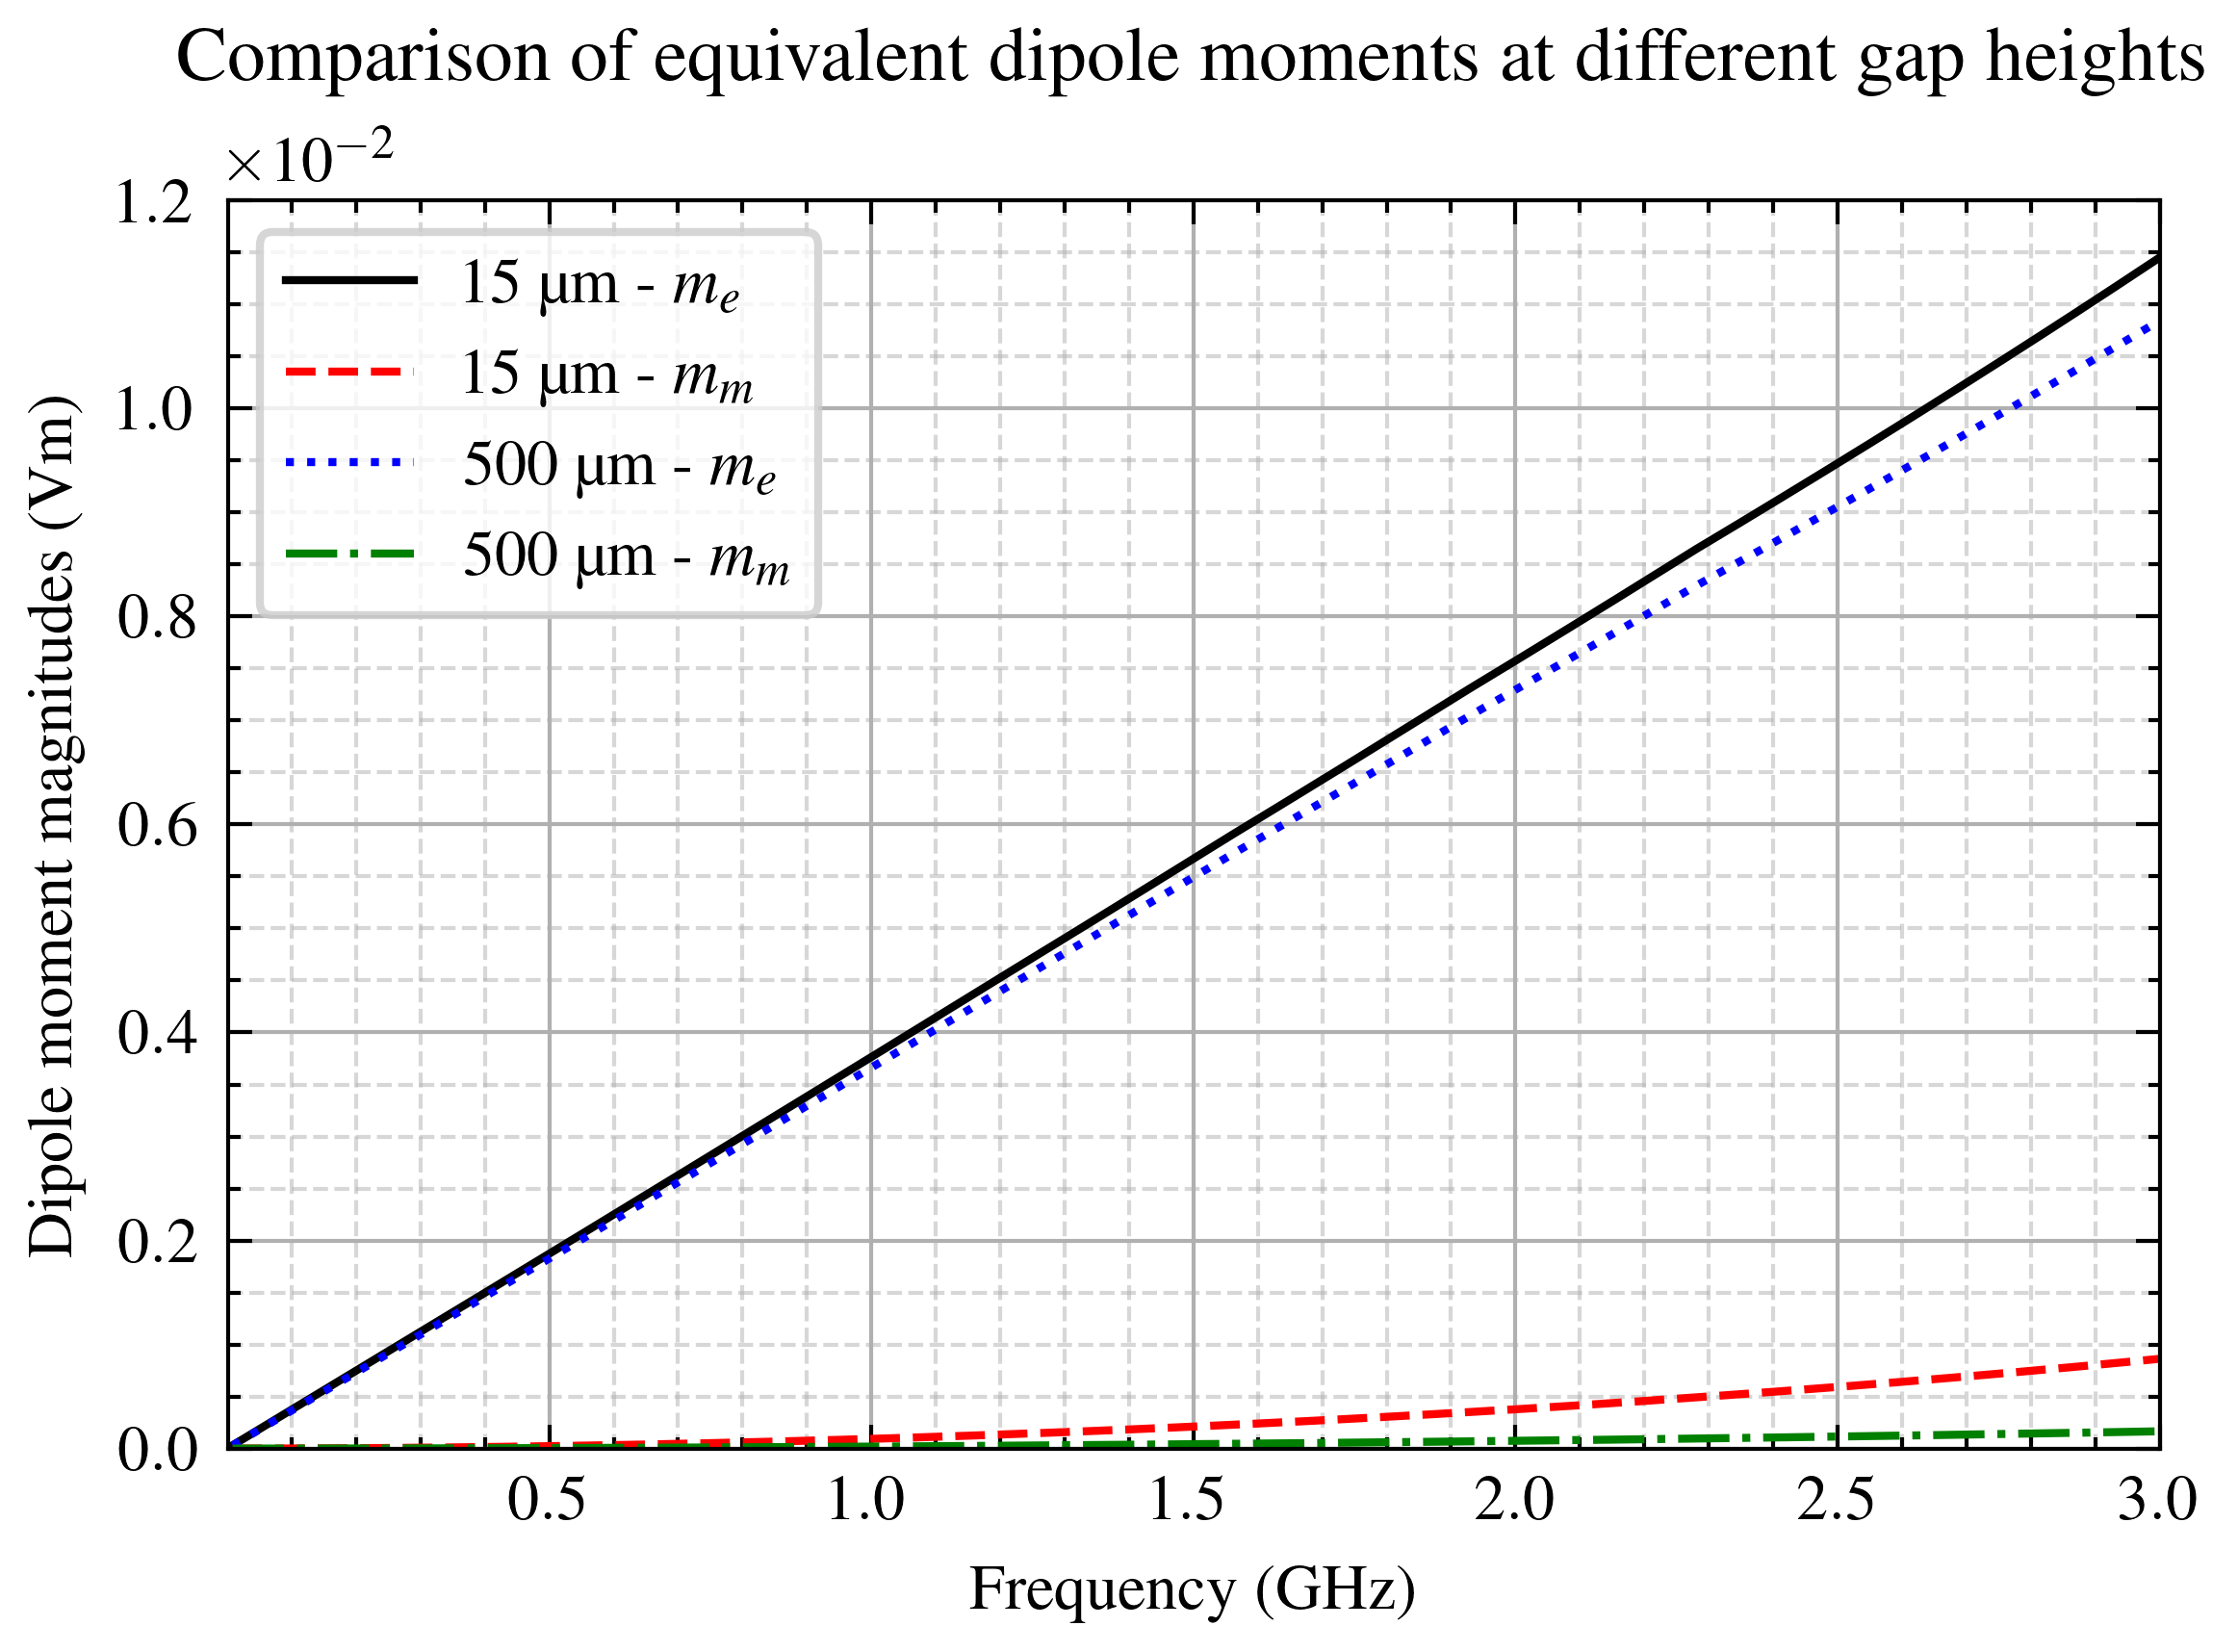
\includegraphics[width=1\linewidth]{content/img/gapped_loop_comp_moments_gap_sweep}
		\caption{Equivalent dipole moments}
		\label{fig:gappedloopcompmomentsgapsweep}
	\end{subfigure}
	\hfill
	\begin{subfigure}[b]{0.48\textwidth}
		\centering
		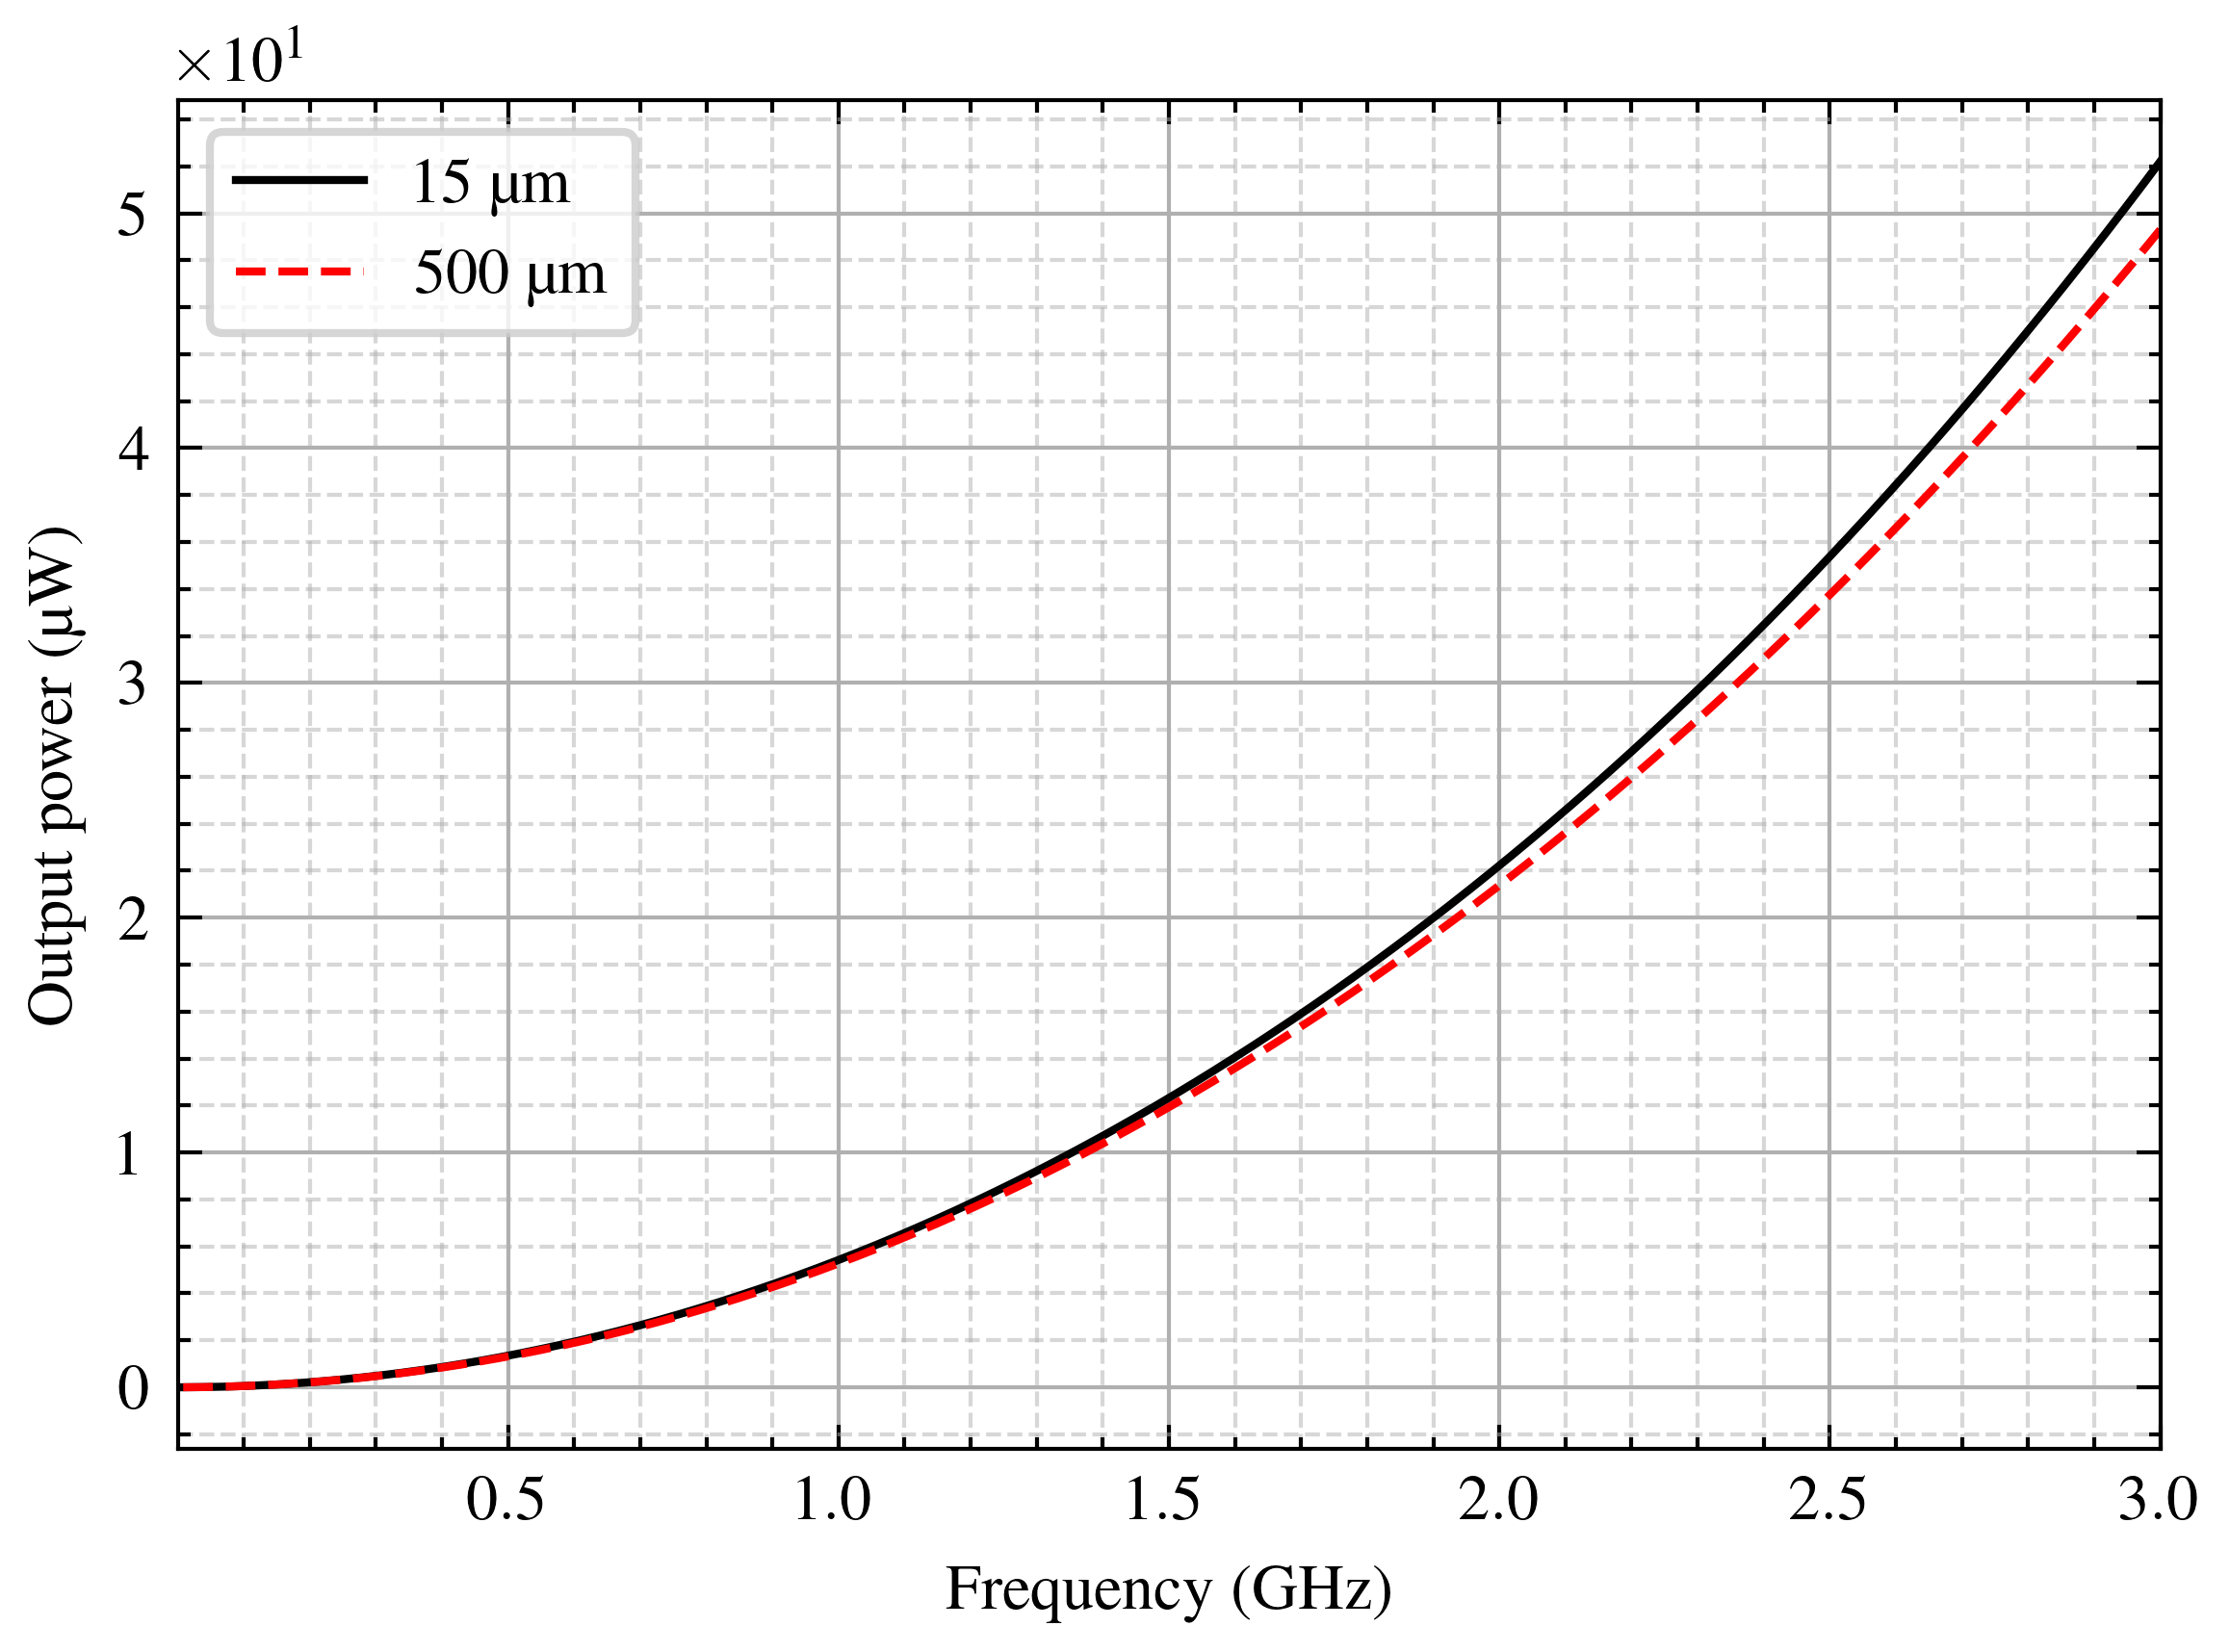
\includegraphics[width=1\linewidth]{content/img/gapped_loop_comp_power_gap_sweep}
		\caption{Output power}
		\label{fig:gappedloopcomppowergapsweep}
	\end{subfigure}
	
	\caption{(a) Comparison of the equivalent dipole moments, where the electric dipole moment $\mathbf{m}_e$ is weighted by $\eta_0$ to allow direct comparison with $\mathbf{m}_m$. (b) Comparison of the output power for different gap heights of the loop antenna.}
	\label{fig:gaplopsweep}
\end{figure}

It is further noted that the increased charge accumulation at the gap boundaries is naturally accompanied by a growing conductive current, as the displacement current rises accordingly. Consequently, an increase in $\mathbf{m}_e$ inherently gives rise to a corresponding increase in $\mathbf{m}_m$.

The input impedance of the loop antenna with gap is capacitive, as confirmed by \autoref{fig:gappedloopimp}. However, in contrast to the monopole antenna, the loop antenna with gap retains a non-negligible inductance due to its closed wire geometry. This is reflected in a more pronounced magnetic dipole moment $\mathbf{m}_m$ and a steeper decline of the impedance magnitude with frequency compared to that of the monopole antenna, shown in \autoref{fig:monopoleimp}.

The feedpoint voltage of the loop antenna with gap decreases slightly more rapidly with frequency than that of the monopole antenna, as shown in \cref{fig:gap-loop-voltage-current}. This subtle difference is attributable to the non-negligible inductance of the closed wire geometry, which induces a voltage that partially couples to the septum and gives rise to $\mathbf{m}_m$ according to \eqref{eqn:m_v}. Nevertheless, the overall voltage behavior remains dominated by the capacitive impedance of the antenna, consistent with the analysis in \cref{sec:monopole}.

The feed current, by contrast, increases more slowly with frequency than in the monopole case, resulting in a correspondingly slower growth of the electric dipole moment $\mathbf{m}_e$ according to \eqref{eqn:me_i}. As a consequence, the magnitude of $\mathbf{m}_e$ remains smaller than that of the monopole antenna across the investigated frequency range, as can be verified by comparing \autoref{fig:gappedloopmoments} with \autoref{fig:dipolemomentsmonopolewide}.

\begin{figure}[htbp]
	\centering
	\begin{subfigure}[b]{0.48\textwidth}
		\centering
		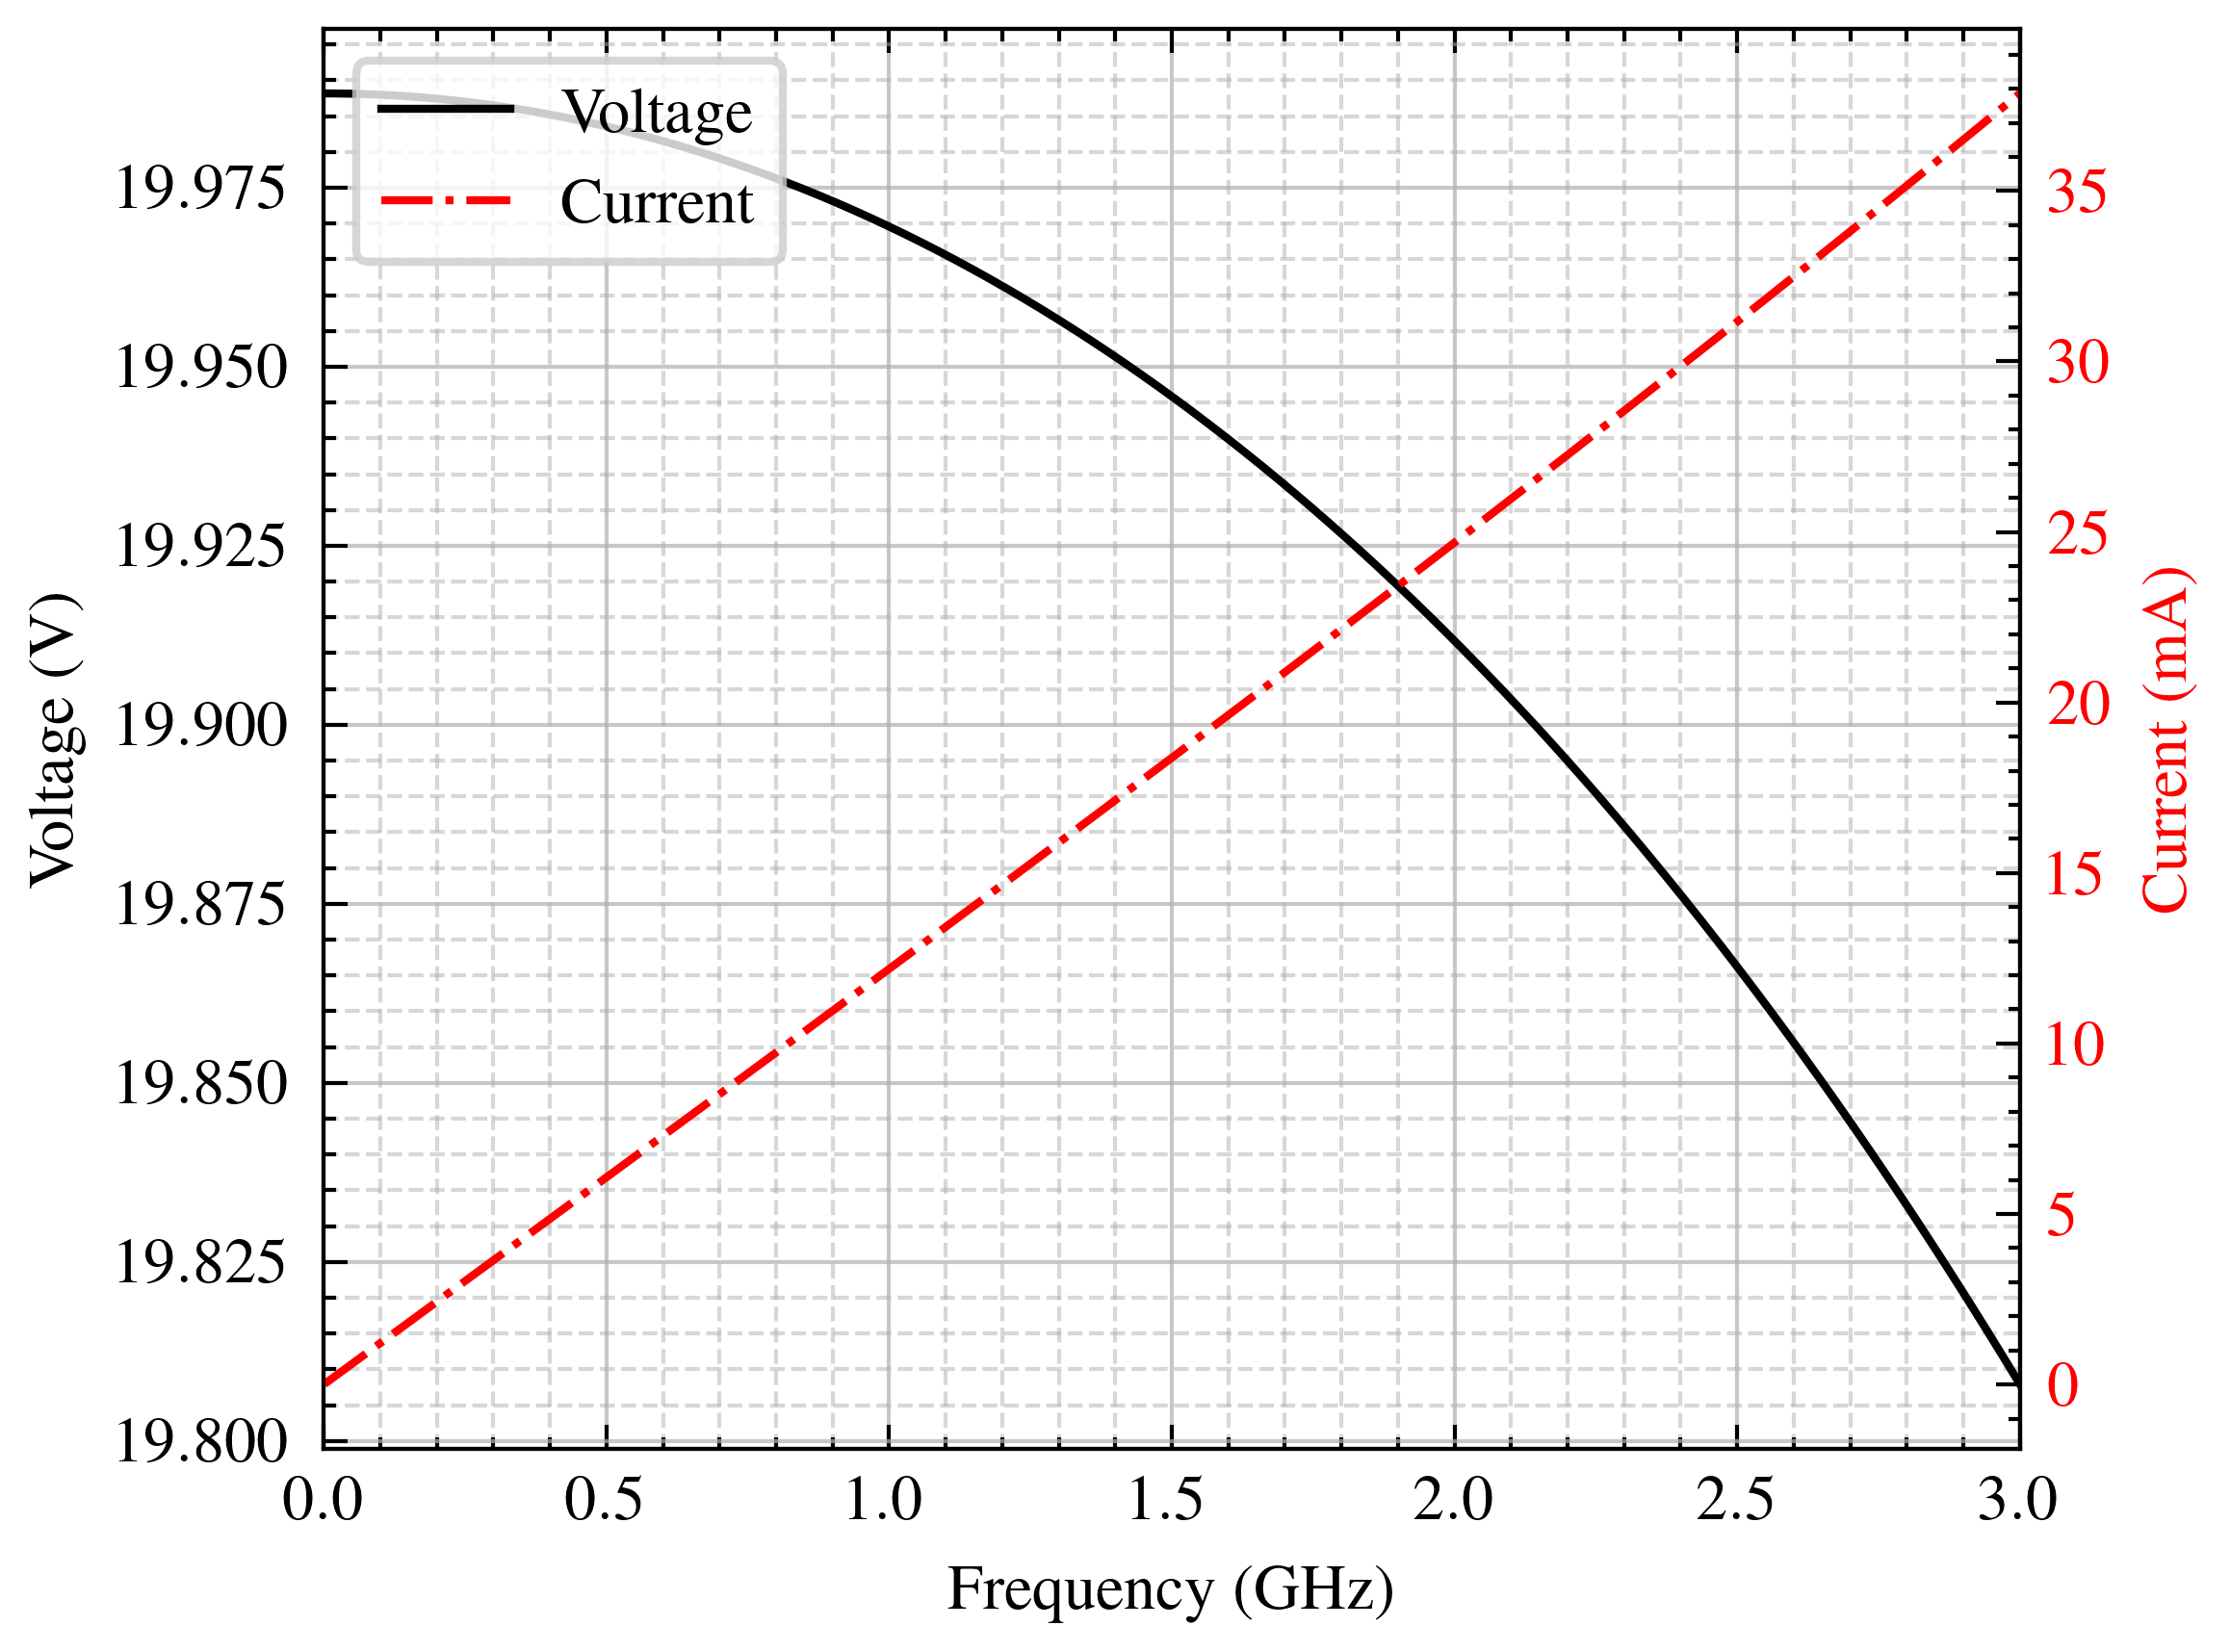
\includegraphics[width=1\linewidth]{content/img/gap-loop-voltage-current}
		\caption{Voltage and current across feedpoint}
		\label{fig:gap-loop-voltage-current}
	\end{subfigure}
	\hfill
	\begin{subfigure}[b]{0.48\textwidth}
		\centering
		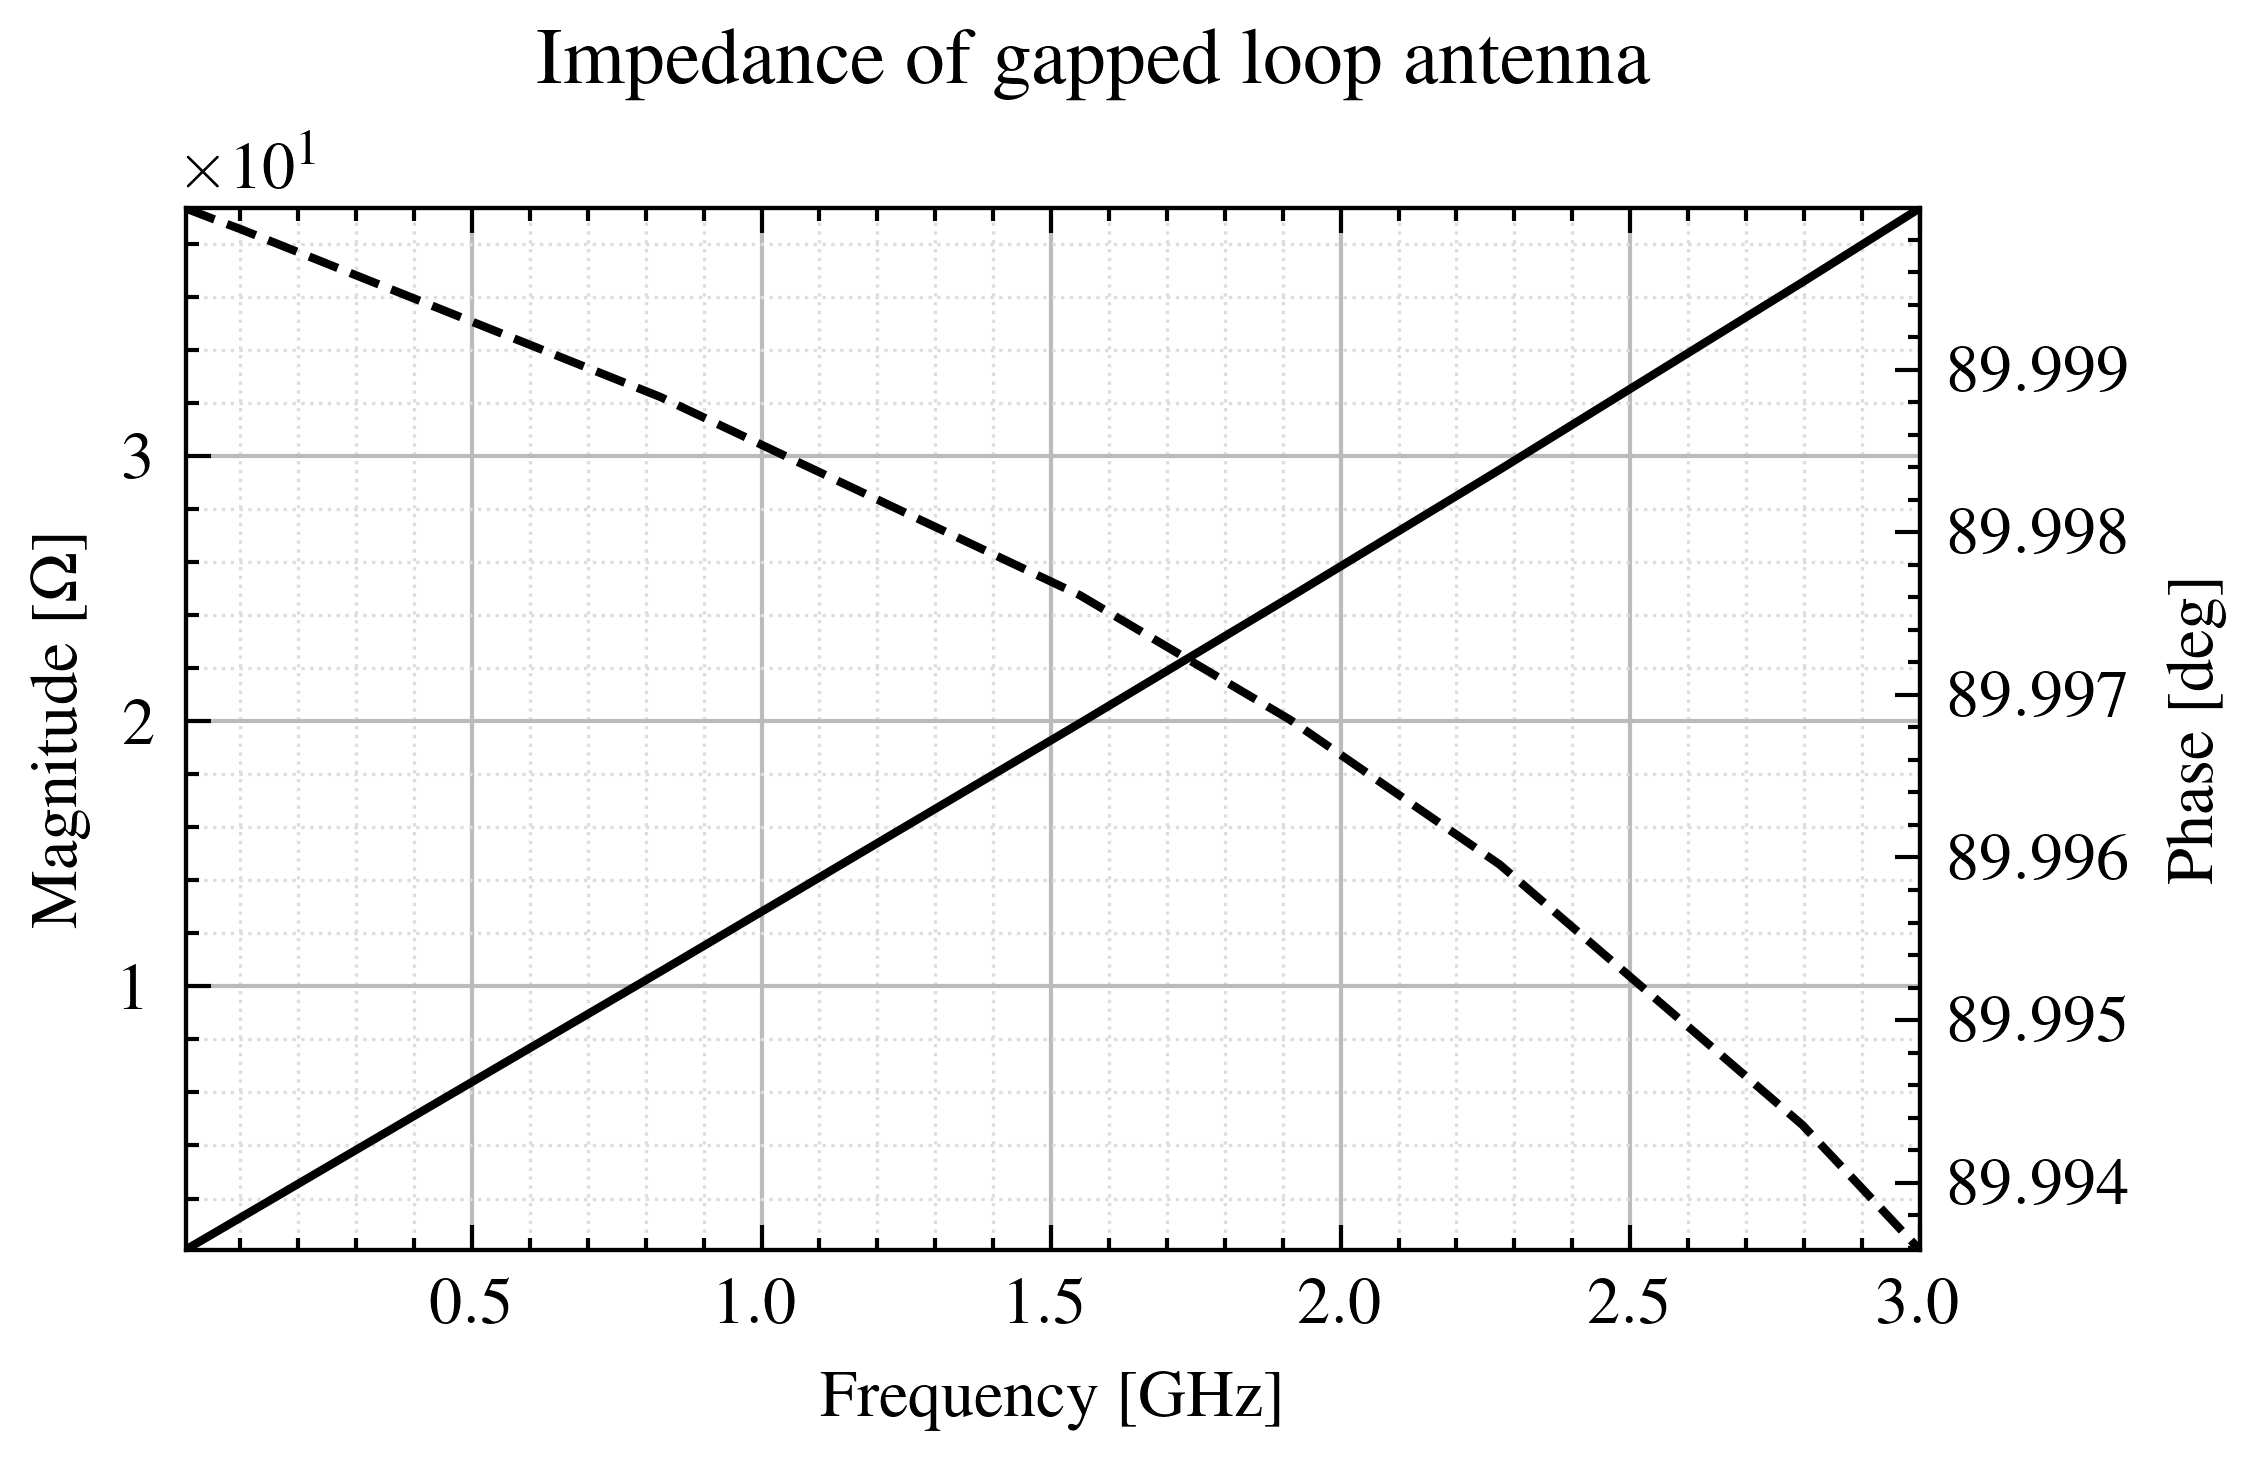
\includegraphics[width=1\linewidth]{content/img/gapped_loop_imp}
		\caption{Magnitude and phase of impedance}
		\label{fig:gappedloopimp}
	\end{subfigure}
	\caption{The voltage and current across the feedpoint in (a), together with the related impedance in (b) of the loop antenna with gap.}
	\label{fig:gapelec}
\end{figure}

In summary, the loop antenna with gap demonstrates that introducing a discontinuity in the return path shifts the antenna toward capacitive behavior, producing equivalent dipole moments analogous to those of the monopole antenna, while retaining a residual magnetic dipole moment whose magnitude is governed by the gap height.
